\documentclass[12pt]{article}
\usepackage{graphics}
\begin{document}

\section*{NYU Physics 1---In-class Exam 4}

\vfill

\paragraph{Name:} ~

\paragraph{email:} ~

\paragraph{recitation:} ~

\vfill

This exam consists of two problems.  Write only in this booklet.  Be
sure to show your work.

\vfill ~

\clearpage

\section*{Problem 1}

As a physics demonstration, NYU decides to hang a $M=50~\mathrm{kg}$
pendulum bob from the roof of Bobst Library, by a light cable, in the
10-story-tall lobby.

(a) If the cable is 10 stories long, what is the approximate period
$T$ you expect for the oscillations of this pendulum?  Give your answer
in s.

\vfill

(b) If the pendulum is set swinging with a horizontal amplitude of
5~m, how much total mechanical energy $E$ is stored in the
oscillation?  Show your work and give your answer in J.

\vfill

(c) What is the maximum horizontal speed $v_\mathrm{max}$ of the
pendulum bob swinging with this amplitude?  Give your answer in
$\mathrm{m\,s^{-1}}$.

\vfill ~

\clearpage

\section*{Problem 2}

The figure shows the potential energy $U(x)$ as a function of position
$x$ for some physical system.
\\ \rule{0.2\textwidth}{0pt}
\resizebox{0.6\textwidth}{!}{\includegraphics{../pro/spring_potential_prob.eps}}

(a) What is the equilibrium position $x_0$?

\vfill

(b) What is the effective ``spring constant'' $k_\mathrm{eff}$ you
might associate with this system?  Give your answer in
$\mathrm{N\,m^{-1}}$.

\vfill ~

\clearpage

[This page intentionally left blank for calculations or other work.]

\end{document}
